\documentclass[]{article}
\usepackage{lmodern}
\usepackage{amssymb,amsmath}
\usepackage{ifxetex,ifluatex}
\usepackage{fixltx2e} % provides \textsubscript
\ifnum 0\ifxetex 1\fi\ifluatex 1\fi=0 % if pdftex
  \usepackage[T1]{fontenc}
  \usepackage[utf8]{inputenc}
\else % if luatex or xelatex
  \ifxetex
    \usepackage{mathspec}
  \else
    \usepackage{fontspec}
  \fi
  \defaultfontfeatures{Ligatures=TeX,Scale=MatchLowercase}
\fi
% use upquote if available, for straight quotes in verbatim environments
\IfFileExists{upquote.sty}{\usepackage{upquote}}{}
% use microtype if available
\IfFileExists{microtype.sty}{%
\usepackage{microtype}
\UseMicrotypeSet[protrusion]{basicmath} % disable protrusion for tt fonts
}{}
\usepackage[top=3cm,left=3cm,right=3cm]{geometry}
\usepackage{hyperref}
\hypersetup{unicode=true,
            pdftitle={Disease Modeling},
            pdfborder={0 0 0},
            breaklinks=true}
\urlstyle{same}  % don't use monospace font for urls
\usepackage{graphicx,grffile}
\makeatletter
\def\maxwidth{\ifdim\Gin@nat@width>\linewidth\linewidth\else\Gin@nat@width\fi}
\def\maxheight{\ifdim\Gin@nat@height>\textheight\textheight\else\Gin@nat@height\fi}
\makeatother
% Scale images if necessary, so that they will not overflow the page
% margins by default, and it is still possible to overwrite the defaults
% using explicit options in \includegraphics[width, height, ...]{}
\setkeys{Gin}{width=\maxwidth,height=\maxheight,keepaspectratio}
\IfFileExists{parskip.sty}{%
\usepackage{parskip}
}{% else
\setlength{\parindent}{0pt}
\setlength{\parskip}{6pt plus 2pt minus 1pt}
}
\setlength{\emergencystretch}{3em}  % prevent overfull lines
\providecommand{\tightlist}{%
  \setlength{\itemsep}{0pt}\setlength{\parskip}{0pt}}
\setcounter{secnumdepth}{5}
% Redefines (sub)paragraphs to behave more like sections
\ifx\paragraph\undefined\else
\let\oldparagraph\paragraph
\renewcommand{\paragraph}[1]{\oldparagraph{#1}\mbox{}}
\fi
\ifx\subparagraph\undefined\else
\let\oldsubparagraph\subparagraph
\renewcommand{\subparagraph}[1]{\oldsubparagraph{#1}\mbox{}}
\fi

%%% Use protect on footnotes to avoid problems with footnotes in titles
\let\rmarkdownfootnote\footnote%
\def\footnote{\protect\rmarkdownfootnote}

%%% Change title format to be more compact
\usepackage{titling}

% Create subtitle command for use in maketitle
\providecommand{\subtitle}[1]{
  \posttitle{
    \begin{center}\large#1\end{center}
    }
}

\setlength{\droptitle}{-2em}

  \title{Disease Modeling}
    \pretitle{\vspace{\droptitle}\centering\huge}
  \posttitle{\par}
    \author{}
    \preauthor{}\postauthor{}
    \date{}
    \predate{}\postdate{}
  
\usepackage{multirow}
\usepackage{multicol}
\usepackage{booktabs}
\usepackage{xcolor}
\numberwithin{equation}{section}
\counterwithin{figure}{section}
\counterwithin{table}{section}
\usepackage{dcolumn}
\usepackage{rotating}
\usepackage{caption}

\begin{document}
\maketitle

{
\setcounter{tocdepth}{2}
\tableofcontents
}
\hypertarget{intro}{%
\section{Intro}\label{intro}}

Over May 2011, a strain \emph{Escherichia coli} (\emph{E. coli}) caused
an outbreak of severe illness in Germany, with \textasciitilde{}3,950
affected compared with \textasciitilde{}200 cases a year typically seen.
Of those infected 53 died.

In this - we extend a method presented by Held et al.
(\protect\hyperlink{ref-held_two-component_2006}{2006}) for modeling
parameters of infectious disease counts in a Bayesian framework. Their
method models the count data as a branching Poisson process with a
cyclical endemic parameter.

We then extend their model to incorporate a graph.

\hypertarget{comments}{%
\subsection{Comments}\label{comments}}

Expand and metion general ideas of epidemics spreading \& how we model
them (\textasciitilde{}1 page)

\hypertarget{intro-to-two-component-model}{%
\section{Intro to Two-Component
Model}\label{intro-to-two-component-model}}

Held et al. (\protect\hyperlink{ref-held_two-component_2006}{2006})
presents a stochastic model for the statistical analysis of infectious
disease counts that serves as the basis of the theextended graph model.

The two components of the model are a simple Poisson branching process
with autoregressive parameter \(\lambda\) and a seasonal component fit
with a Fourier series. These components are described as the
``epidemic'' and ``endemic'' components respectively. Additionally, the
two-component model allows for the \(\lambda\) to change over time
allowing for the disease to change infectivity over time.

\hypertarget{two-component-model-notation}{%
\subsection{Two-Component Model
Notation}\label{two-component-model-notation}}

Let \(Z = (Z_0, Z_1, ..., Z_n)\) be the infectious disease counts at
each time step \(t\). The model is then specified through
\(Z_t | Z_{t-1}\).

Each \(Z_t\) is determined as

\[ Z_t = Y_t + X_t,\ t\in\{1,\dots, n\}\]

Where \(Y_t\) is the epidemic component and \(X_t\) is the endemic
component. The epidemic component is parameterized as:
\[Y_t|Z_{t-1} \sim Pois(\lambda_tZ_{t-1})\] Where \(\lambda_t\) is
piecewise constant depending on an unknown number of changepoints \(K\)
and unknown locations \(\theta_1 < \cdots < \theta_K\).

\[ \lambda_t =  \begin{cases} \lambda^{(1)} & t < \theta_0 \\
\lambda^{(k)}, & \theta_{k} \leq t < \theta_{(k-1)} \\
\lambda^{(K+1)}, & t \geq \theta_K \end{cases}\]

The endemic component is parameterized as:

\[ X_t \sim Pois(\nu_t)\]

Where \(\log{\nu_t}\) is modeled as a Fourier series:

\[ \log{\nu_t} = \gamma_0 + \sum_{l = 1}^L \big(\gamma_{2l-1}\sin(\rho l t)+\gamma_{2l}cos(\rho l t)\big) \]

\hypertarget{epidemic-component}{%
\subsection{Epidemic Component}\label{epidemic-component}}

The epidemic component is given by:

\[Y_t|Z_{t-1} \sim Pois(\lambda_tZ_{t-1})\]

Where \(\lambda_t\) is the time varing infectivity parameter and
\(Z_{t-1}\) is the the infected count in the previous time step.

We can think of \(\lambda_t\) as the infectivity of the disease at time
\(t\) with an infected person causing new infections as
\(Pois(\lambda_t)\). Since each infected at time \(Z_{t-1}\) generates
new infected i.i.d \(Pois(\lambda_t)\), then \(Z_t\) is the sum of those
random variables which itself is Poisson;
\(\sum_1^{Z_{n-1}}Pois(\lambda_t) = Pois(\lambda_tZ_{n-1})\).

In this model, the \(\lambda_t\) is allowed to vary over time. The
parameter \(\lambda = (\lambda_1,\cdots,\lambda_n)\) is a piecewise
constant function with unknown number of changepoints \(K\) and unknown
location of changepoints \(\theta_1 < \cdots < \theta_K\) with
\(\theta \in \{1,...,n-1\}\). If \(K = 0\) there is no changepoint and
the \(\lambda\) parameter is constant throughout.

\hypertarget{tk-add-references-below}{%
\subsection{TK add references below}\label{tk-add-references-below}}

For constant \(\lambda\), this is known as a Poisson branching process.
For such a process, when \(\lambda > 1\) the process explodes and the
number of infected goes to infinity with probability 1. When
\(\lambda < 1\) then the process ``goes extinct'' or reaches and remains
at 0 with probability 1. Once the process reaches a point where
\(Z_t = 0\), it remains there as there are no more infected to create
new infected at the next time step. When \(\lambda_t > 1\) an
``outbreak'' occurs shown as the spike in the graph between. When
\(\lambda_t < 1\) the outbreak ends.

Allowing \(\lambda_t\) to vary captures many scenarios, for example a
particulary infectious strain of the flu could cause \(\lambda_t\) to
increase above 1 and cause an outbreak. Later, better or new vaccines
and quarentine procedures can cause the overall infectivity to decrease
below 1.

\hypertarget{endemic-component}{%
\subsection{Endemic Component}\label{endemic-component}}

To prevent the branching proccess going extinct or going to infinity,
the model includes an endemic component.

The endemic component is given by:

\[X_t \sim Pois(\nu_t)\]
\[\log{\nu_t} = \gamma_0 + \sum_{l = 1}^L (\gamma_{2l-1}\sin(\rho l t)+\gamma_{2l}cos(\rho l t))\]

That is, \(\log{\nu_t}\) is fit with a Fourier series which can
approximate any function arbitrarily closely. In Held et al.
(\protect\hyperlink{ref-held_two-component_2006}{2006}) they limit
\(L = 1\) since they determined higher order frequencies were
insignificant.

The parameter can then be fit with a linear regression
\(\log{\nu_t} = s_t\gamma^T\)

where
\(s_t = \langle 1, sin(\rho l t), \gamma_{2l}cos(\rho l t) \rangle\)

\begin{figure}
\centering
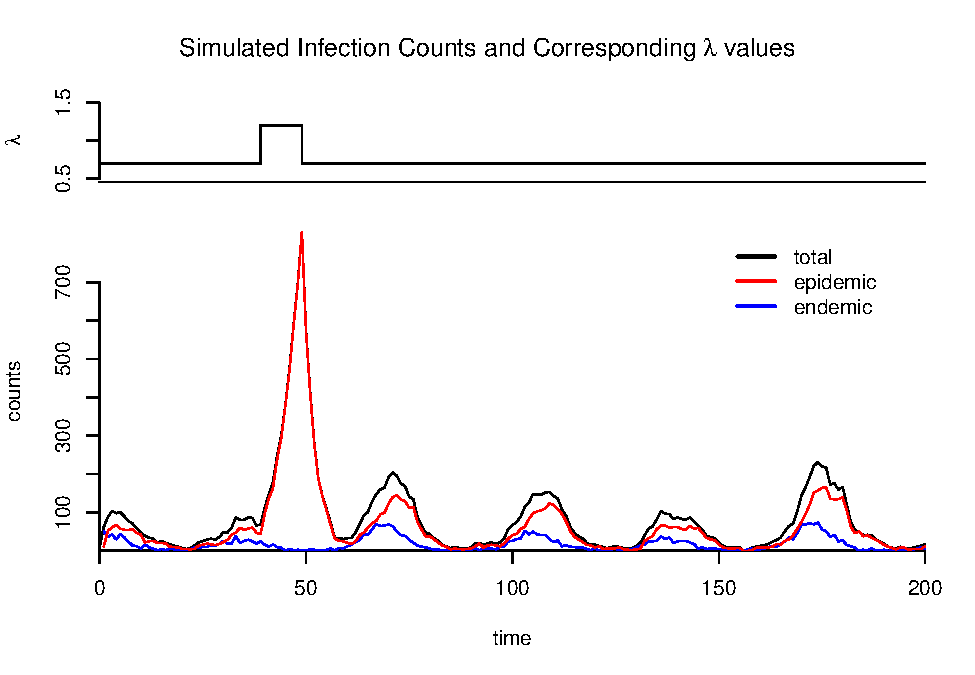
\includegraphics{thesis_draft_files/figure-latex/simulation figure-1.pdf}
\caption{\label{fig:figs}plotting example}
\end{figure}

\hypertarget{actual-model}{%
\section{Actual Model}\label{actual-model}}

\hypertarget{likelihood}{%
\subsection{Likelihood}\label{likelihood}}

\[P(Z|Z_0) = \prod_{t=1}^b P(Z_t|Z_t{-1})\] Where

\[Z_t|Z_{t-1} \sim Pois(\nu_t + \lambda_tZ_{t-1})\]

\[\log{\nu_t} = \gamma_0 +  \gamma_{1}\sin(\rho l t)+\gamma_{2}\cos(\rho l t)\]

\[ \lambda_t =  \begin{cases} \lambda^{(1)} & t < \theta_0 \\
\lambda^{(k)}, & \theta_{k} \leq t < \theta_{(k-1)} \\
\lambda^{(K+1)}, & t \geq \theta_K \end{cases}\]

\hypertarget{priors}{%
\subsection{Priors}\label{priors}}

\[P(K = k) \sim 1/n,\ k \in \{1,\dots,n\}\]
\[P(\theta|K=k) = \binom{n}{k}^{-1}\]

\[\gamma_i \sim N(0, 3I_3), i \in \{0,1,2\}\]

\[ \lambda^{(k)} \sim Gamma(1, 1),\ k \in \{1, \dots, K + 1\} \]

Then the full likelihood is

\[ P(Z_t|Z_{t-1},\theta, K, \lambda^{(1)}, \dots, \lambda^{(K+1)}, \gamma_0, \gamma_1, \gamma_2)*P(\theta|K)*P(K)*P(\prod_{k=1}^{k+1}\lambda^{(k)} )*P(\prod_{i=0}^2 \gamma_i)  \]

\hypertarget{bayesian-inference}{%
\section{Bayesian Inference}\label{bayesian-inference}}

In Bayesian analysis, we aimt to calculate the posterior distribution of
the parameters given the data via Bayes' theorem.

\[ P(\text{parameters}|\text{data}) = \frac{P(\text{data}|\text{parameters})P(\text{parameters})}{P(\text{data})} \]

One issue is the computation of \(P(\text{data})\) which is given by
\(\int P(\text{data}|\text{parameters})P(\text{parameters})\) over the
entire parameter space. With many parameters this integral it typically
analytically intractable. To deal with this issue ({\textbf{???}})
writes many of the distributions as conjugate priors etc (tk elaborate)
and uses Markov Chain Monte-Carlo (MCMC) methods for some.

In this work we primarily appeal to MCMC methods.

\hypertarget{markov-chain-monte-carlo}{%
\subsection{Markov chain Monte-Carlo}\label{markov-chain-monte-carlo}}

(tk terrible explanation)

A Markov Chain is a sequence of random variables \((X_n)\) where
\(P(X_n)\) depends only on \(X_{n-1}\).

A probability distribution on the states of a Markov Chain is said to be
a stationary distribution \(\pi\) i

That is a distribution \(\pi\) is a stationary distribution of the
Markov Chain with transition probabilities \(P\) if

\[ \pi = \pi P \]

In Markov chain Monte Carlo (MCMC), the algorithm generates samples from
a given posterior dist \(\pi\) by constructing a Markov chain with
stationary distribution \(\pi\)

One method for constructing the chain is the Metropolis-Hastings
Algorithm

\hypertarget{metropolis-hastings-aglorithm}{%
\subsection{Metropolis-Hastings
Aglorithm}\label{metropolis-hastings-aglorithm}}

We start with a Markov Chain with proposal distribution \(q(i,j)\).

We then modify \(q\) in the following way to obtain a Markov Chain with
stationary distribution \(\pi\).

\begin{enumerate}
\def\labelenumi{\arabic{enumi}.}
\tightlist
\item
  From the current state \(X_n = i\) propose a new state \(j\) according
  to \(q\).
\item
  Compute the acceptance probability
\end{enumerate}

\[a(i,j) = \min{\big(\frac{\pi(j)q(j,i)}{\pi(i)q(i,j)},1\big) }\]

\begin{enumerate}
\def\labelenumi{\arabic{enumi}.}
\setcounter{enumi}{2}
\tightlist
\item
  Generate \(U \sim Unif(0,1)\)
\item
  If \(U < a_{ij}\) then accept the move and \(X_n = j\) otherwise
  reject and \(X_n = i\).
\end{enumerate}

This new Markov Chain has a transition probability

\[p(i,j) = q(i,j)a(i,j)\]

Assuming \(a(i,j) < 1\)

\[ \begin{aligned} \int \pi(i)*p(i,j) & = \int\pi(j)*p(j,i) \\
\int \pi(i)q(i,j)\frac{\pi(j)q(j,i)}{\pi(i)q(i,j)} & = \int\pi(j)*q(j,i)*a(j,i) \\ \int \pi(j)*q(j,i)*1 & = \int\pi(j)*q(j,i)*a(j,i)
\end{aligned}\]

\hypertarget{reversible-jump-mcmc}{%
\subsection{Reversible Jump MCMC}\label{reversible-jump-mcmc}}

To handle the dimension jumping of the model (between different number
of changepoints) we use Reversible Jump MCMC.

Since the model can jump between a collection of possible models
\(\{M_k, k \in \{0,1,\cdots,n-1\}\}\) where \(k\) indexes the number of
possible changepoints.

The issue comes from the fact that we can only compare points in the
parameter space if they're defined on the same probability space.

To properly do so we need to use a Reversible Jump MCMC.

The procedure is as follows:

\begin{enumerate}
\def\labelenumi{\arabic{enumi}.}
\tightlist
\item
  Draw \(u \sim Unif(0,1)\)
\item
  The following proposals for the new \(\lambda\) values are from
\end{enumerate}

\[\lambda*(\frac{u}{1-u})^{(\theta_1-\theta_0)/(\theta_2-\theta_0)}\]
\[\lambda*(\frac{1-u}{u})^{(\theta_2-\theta_1)/(\theta_2-\theta_0)}\]

That is the new \(\lambda\) values are a compromise between the original
value as a function of where the new changepoint is factored in.

\begin{enumerate}
\def\labelenumi{\arabic{enumi}.}
\setcounter{enumi}{2}
\tightlist
\item
  Acceptance probability; In order to determine the acceptance
  probability for the proposal, the corresponding death move must also
  be determined.
\end{enumerate}

This is done deterministically such that if the newly proposed
changepoint is removed (and the heights were the same as newly proposed
ones), then the new height should be the original height.

Then the new proposal probability would be

\[ \frac{p({K+1 \rightarrow K})*\frac{1}{K+1}}{p(K\rightarrow K+1)*\frac{1}{N-K}} \]
and the Jacobian is given by

\[(\lambda_1 + \lambda_2)^2/\lambda_0\]

\texttt{death\_theta()} a Reversilbe Jump MCMC

\hypertarget{implementation}{%
\section{Implementation}\label{implementation}}

\hypertarget{proposals}{%
\subsection{Proposals}\label{proposals}}

Gamma, \(\lambda\) are updated in respective blocks with a random walk
metropolis.

The number of changepoints \(K\) is updated by either randomly adding a
new changepoint or by randomly deleting a current changepoint. This is
done via a Reversible Jump MCMC

\hypertarget{graph-notation}{%
\section{graph notation}\label{graph-notation}}

We now represent with

\[X_{it}: \text{infected count in city } i \text{ at time step } t \text{, due to endemic factors}   \]
\[Y_{it} : \text{infected count in city } i \text{ at time step } t \text{, due to epidemic factors}   \]

\[Z_{i,t+1} = X_{i,t} + Y_{i,t}: \text{infected count in city } i \text{ at time step } t \]
We have: \[X_{i,t} \sim Pois(\nu_t)\]

\[Y_{i,t}|G \sim ~ Pois\big(\lambda_t*\sum_{j=1}^nZ_{i,t}1[e_{i,j}=1]\big) \]

Where

\[Y_{i,t} |G =   1[e_{1,i}]Z_{1,t-1} + 1[e_{2,i}]Z_{2,t-1} + \cdots + 1[e_{n,i}]Z_{1,t-1} | G  \]

\[P(G) \sim ERGM(\beta_0,\beta_1,...\beta_i)| \beta_0,\beta_1,...\beta_i\]

Where the \(\beta_i\) are covariates assuming dyadic independence.

So the probability of \(logit[P(G_{ij} = 1)] = X^T\beta\)

\hypertarget{citations}{%
\section*{Citations}\label{citations}}
\addcontentsline{toc}{section}{Citations}

\hypertarget{refs}{}
\leavevmode\hypertarget{ref-held_two-component_2006}{}%
Held, Leonhard, Mathias Hofmann, Michael Höhle, and Volker Schmid. 2006.
``A Two-Component Model for Counts of Infectious Diseases.''
\emph{Biostatistics} 7 (3): 422--37.
\url{https://doi.org/10.1093/biostatistics/kxj016}.


\end{document}
